%% content.tex
%%

%% ==============
\chapter{Content Chapters}
\label{ch:Content1}
%% ==============

The content chapters of your thesis should of course be renamed. How many chapters you need to write depends on your thesis and cannot be said in general.


\section{Section 1}

\dots

\subsection{Subsection 1}

\dots

\subsubsection{Subsubsection 1}

\dots

\paragraph{Paragraph 1}

\dots

\subparagraph{Subparagraph 1} Always reference figures, tables etc. To give a few simple examples, this section contains Algorithm \ref{theorem:doof}, Table \ref{tbl:randomnumbers}, Figure \ref{fig:somegraph}, and Theorem \ref{theorem:doof}. To give an example citation we recommend the book of Garey and Johnson \cite{gj-ci-79}.

\begin{theorem}
\label{theorem:doof}
  Wer das liest ist doof.
\end{theorem}
\begin{proof}
  Weil ist so.
\end{proof}

\begin{algorithm}[bt]
\caption{\textsc{Dijkstra}}\label{alg:dijkstra}

% Some settings
\DontPrintSemicolon %dontprintsemicolon
\SetFuncSty{textsc}
\SetKwFor{ForAll}{forall}{do}

% Declaration of data containers and functions
\SetKwData{Q}{Q}
\SetKwData{dist}{d}
\SetKwData{pred}{pred}
\SetKwFunction{queueDeleteMin}{deleteMin}
\SetKwFunction{queueInsert}{insert}
\SetKwFunction{queueDecreaseKey}{decreaseKey}
\SetKwFunction{queueContains}{contains}

% Algorithm interface
\KwIn{Graph $G = (V,E,\omega)$, source node $s$}
\KwData{Priority queue \Q}
\KwOut{Distances \dist{$v$} for all $v \in V$, shortest-path tree of $s$ given by \pred{$\cdot$}}

% The algorithm
\BlankLine
\tcp{Initialization}
\ForAll{$v \in V$}{$\dist{v} \leftarrow \infty$ \; $\pred{v} \leftarrow \texttt{null}$}
\Q.\queueInsert{$s,0$}\; $\dist{s} \leftarrow 0$ \;
\BlankLine
\tcp{Main loop}
\While{\Q is not empty}
{
  $u \leftarrow$ \Q.\queueDeleteMin{} \;
  \ForAll{ $(u,v) \in E$ }
  {
    \If{$\dist{u} + \omega(u,v) < \dist{v}$}
    {
      $\dist{v} \leftarrow \dist{u} + \omega(u,v)$ \;
      $\pred{v} \leftarrow u$ \;
      \uIf{\Q.\queueContains{v}}
      {
        \Q.\queueDecreaseKey{$v, \dist{v}$}
      }
      \Else
      {
        \Q.\queueInsert{$v, \dist{v}$}
      }
    }
  }
}
\end{algorithm}

\begin{table} [bt]
\centering
\caption{Some strange numbers.}
\begin{tabular}{rr}
\toprule
First column & Second column \\
\midrule
3\,109\,218\,136 & 3\,208\,415\,108 \\
2\,231\,385\,058 & 1\,959\,477\,358 \\
1\,287\,719\,872 & 1\,317\,165\,206 \\
2\,516\,844\,936 & 2\,630\,583\,944 \\
1\,569\,466\,774 & 1\,636\,507\,220 \\
1\,032\,627\,816 &    991\,322\,491 \\
\bottomrule
\end{tabular}
\label{tbl:randomnumbers}
\end{table}

\begin{figure} [bt]
  \centering
  \tikzstyle{node}=[circle,inner sep=0.5mm,minimum size=5.25mm,draw = black]
\tikzstyle{bright}=[fill=black!14]
\tikzstyle{dark}=[fill=black!28]
\tikzstyle{lightEdgeStyle}=[black!20]

\newcommand{\numberOfNodes}{5} % must be >= 4

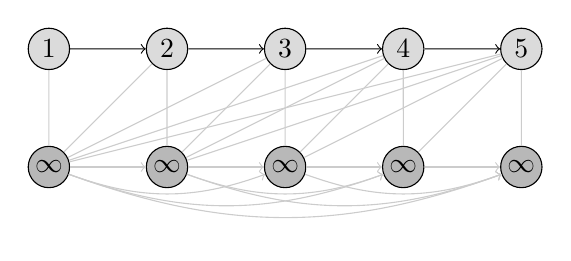
\begin{tikzpicture}[scale=1.5, bend angle = 20]

% Obere Reihe
\node(Top1) at (1,1) [node, bright] {1};
\foreach \i [evaluate = \i as \lastNode using \i-1] in {2,3,...,\numberOfNodes}
{
  \node (Top\i) at (\i,1) [node, bright] {\i}
    edge[<-] (Top\lastNode);
}

% Untere Reihe
\node(Bot1) at (1,0) [node, dark] {$\infty$};
\foreach \i [evaluate = \i as \lastNode using \i-1] in {2,3,...,\numberOfNodes}
{
  \node (Bot\i) at (\i,0) [node, dark] {$\infty$}
    edge[<-, lightEdgeStyle] (Bot\lastNode);
}

% Kanten zwischen den Reihen
\foreach \i in {1,2,...,\numberOfNodes}
{
  \foreach \j in {\i,...,\numberOfNodes}
   {
     \draw[lightEdgeStyle] (Bot\i) -- (Top\j);
   }
}

% Pfeile nach rechts
\pgfmathparse{\numberOfNodes - 2}
\foreach \i [evaluate = \i as \nextNode using \i+2] in {1,2,...,\pgfmathresult}
{
 \foreach \j [count=\nodeIndex from \nextNode] in {\nextNode,...,\numberOfNodes}
 {
   \draw[->, lightEdgeStyle] (Bot\i) to [bend right] (Bot\nodeIndex);
 }
}

\end{tikzpicture} 
 % for .pdf files etc use \includegraphics{test.pdf}
  \caption{A funny graph.}
  \label{fig:somegraph}
\end{figure}
